\documentclass[a4paper,10pt,hidelinks]{article}

\usepackage[margin=2cm]{geometry}

\usepackage{tikz}
\usepackage{hyperref}
\usepackage{algorithm}
\usepackage{algpseudocode}
\usepackage{amsmath}

\usepackage{listings}
\lstset{
    numbers=left,
    breaklines=true,
    tabsize=4
}

\newcommand{\algorithmautorefname}{Algorithm}

%opening
\title{Practical Assignment 2\\
Social Network Analysis}
\author{Bert Peters\\
s1147919}

\begin{document}

\maketitle

\section{Clustering Coefficient}

\begin{enumerate}
 \item A tree, by definition, has no loops, and therefore has a clustering coefficient of 0. Another example is a bipartite graph. This type of graph can only have cycles of at least length 4. This is because it is impossible for two edges in the same partition to have a connection. Cycles of length 4 do not contribute to the clustering coefficient, because that only counts the number of triangles, i.e. the number of cycles of length 3.

 \item There are several possible such graphs. One of them is shown in \autoref{fig:graph-no-clustering}.
 
 \item Contructing an unclustered graph is trivial for when $m \leq n$, because we can construct a circle graph of size $n$ and remove edges to arrive at the desired number of edges. The algorithm is shown in \autoref{algo:algo-no-clustering} and runs in $O(m)$.
 
The algorithm works by adding repeatedly connecting each node $v_i$ to another node $v_{i + \delta}$. This delta is increased over iterations, and is given by $\delta = 3^s$ where $s$ is the current iteration number, starting at 1. This ensures that we do not create new loops shorter than 4, which is what we need in order to prevent clustering.
\end{enumerate}

\begin{figure}
    \centering
    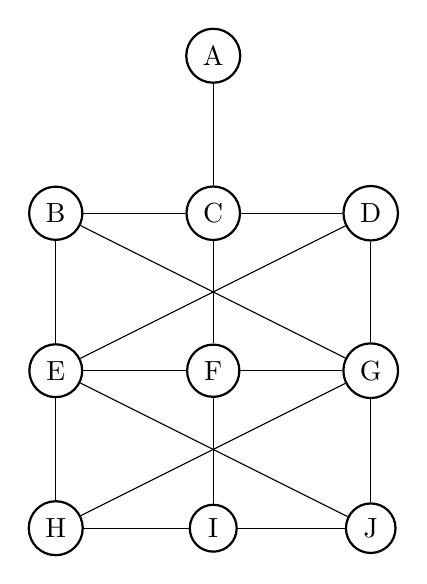
\begin{tikzpicture}[every node/.style={draw=black,thick,circle}]
        \node (A) at (0,4){A};
        \node (B) at (-2,2){B};
        \node (C) at (0,2){C};
        \node (D) at (2,2){D};
        \node (E) at (-2,0){E};
        \node (F) at (0,0){F};
        \node (G) at (2,0){G};
        \node (H) at (-2,-2){H};
        \node (I) at (0,-2){I};
        \node (J) at (2,-2){J};
        
        \draw (A) -- (C);
        \draw (B) -- (C);
        \draw (C) -- (D);
        \draw (B) -- (E);
        \draw (C) -- (F);
        \draw (E) -- (F);
        \draw (D) -- (G);
        \draw (F) -- (G);
        \draw (E) -- (H);
        \draw (H) -- (I);
        \draw (F) -- (I);
        \draw (I) -- (J);
        \draw (G) -- (J);
        
        \draw (B) -- (G);
        \draw (D) -- (E);
        
        \draw (E) -- (J);
        \draw (G) -- (H);

    \end{tikzpicture}
    \caption{An undirected graph with 10 nodes, 15 edges, and a clustering coefficient of 0.}
    \label{fig:graph-no-clustering}
\end{figure}

\begin{algorithm}
\caption{Constructing a graph with no clustering.}
\label{algo:algo-no-clustering}

\begin{algorithmic}
    \State $E \gets \emptyset$
    \State $s \gets 1$
    \While{$|E| < m \land 3^s < n$}
    		\For{$v_i \in V \land |E| < m$}
    			\State $E \gets E \cup \{\{v_i, v_{i + 3^s \text{ mod } n} \}\}$
    		\EndFor
    		\State $s \gets s + 1$
    \EndWhile
\end{algorithmic}

\end{algorithm}

\section{Densest Subgraph}

We start by computing the average degree and the current density. For a graph with a given $n, m$ this is easy, because the average degree is $\frac{2m}{n}$ and the density is half of that. We run our algortihm, by iteratively removing the nodes with a degree lower than the average degree from our $V$ and $E$, and repeat the process until we cannot delete nodes anymore.

Using the above algorithm, we arrive at the results as shown in \autoref{tab:densest-subgraph}. We see that after iteration 1, we already find our maximum, with a density of 1.5. After that, we still delete nodes twice, until we arrive at a graph with two nodes and cannot delete nodes anymore.

\begin{table}
    \centering
    \begin{tabular}{r || l | r | r}
        Iteration & Subgraph & Density & Avg. degree\\
        \hline
        0   & $\{A B C D E F H I J K L\}$ & $\frac{16}{11} \approx 1.45 $ & $\frac{32}{11} \approx 2.9 $ \\
        1   & $\{A B E F J K\}$ & $ \frac{9}{6} = 1.5 $ & $ \frac{18}{6} = 3 $ \\
        2   & $\{B E F J\}$ & $\frac{5}{4} = 1.25$ & $\frac{10}{4} = 2.5$ \\
        3   & $\{E F\}$ & $\frac{1}{2} = 0.5$ & $\frac{2}{2} = 1$
    \end{tabular}
    \caption{Using the greedy algorithm to find the densest subgraph.}
    \label{tab:densest-subgraph}
\end{table}

\section{Twitter Network Extraction}



\subsection{Parsing the tweets}

We parse the tweets using a python script in \autoref{lst:preprocess}. It takes a list of files as arguments from the command line or data from the standard input. First, it splits the string twice on the first occurrence of a tab. It attempts to parse mentions out of a tweet using a regular expression. The expression used is a non-word character\footnote{A word character is defined as either an ascii letter character (upper case and lower case), a digit, or an underscore character (`\texttt{\_}'). Everything else, including the `\texttt{\^}' (start of string) and `\texttt{\$}' (end of string) metacharacters is considered a non-word character.}, followed by an `\texttt{@}', followed by $[1, 15]$ word characters\footnote{The specification of what is a valid twitter username can be found at \url{https://support.twitter.com/articles/101299}}, followed by by a non-word character. Requiring a non-word character before the mention filters out email addresses, which occur frequently in the dataset. The resulting usernames are put in lowercase, because twitter usernames are case-insensitive.

The script determines a mapping from usernames to integers, because this is more convenient to handle programmatically in the analysis. It outputs a Gephi-edgelist compatible list of mentions to the standard output, and a Gephi-nodelist compatible username mapping to the standard error.

There are still a number of things that the parser does wrong. The most prevalent error happens when users have no separator (either white space or punctuation) between a mention and the following text. In this case, it is impossible to determine where the username ends and the tweet continues. This can only be solved when you know all usernames in your dataset.

This problems described above can, however, be solved by using the twitter api. It provides any mentions included in a message as meta data, removing the need for complicated parsers. Implementing this is outside the scope of this assignment.

\subsection{Dataset statistics}

We consider the graph as an undirected graph. We use our parser program to get some statistics about our dataset. The results are shown in \autoref{tab:dataset-stats}. For the degree distribution, we reuse the python script from the previous assignment. This gives us the distribution as shown in \autoref{fig:graph-no-clustering}.

Edges occurring multiple times are counted towards node degrees, but not towards the number of edges. In other words, the equation $\sum\limits_{v_i} k(v_i) = 2|V|$ does not hold.

For density, we take the measure $D = \frac{|V|}{|E|(|E| - 1)}$. Since, in a social network, the average degree does not depend on the number of nodes in the network, we we expect the density to drop linearly with the number of nodes. This is because $\lim_{n \rightarrow \infty} \frac{cn}{n (n - 1)} = \frac{1}{n}$. Furthermore, there should be a slightly lower  density in the entire network and that in the giant component. This is because the network contains a lot of isolated nodes, i.e. people that have tweeted, but not mentioned, and who have not been mentioned.

\begin{table}
	\centering
	\begin{tabular}{l || r | r | c | r | r | c}
	Dataset & $|V|$ & $|E|$ & $D$ & $|V_{giant}|$ & $|E_{giant}|$ & $D_{giant}$ \\
	\hline
	\texttt{twitter-small} & 47972 & 54517 & $2.4 \cdot 10^{-5}$ & 32864 & 45171 & $4.2 \cdot 10^{-5}$ \\
	\texttt{twitter-larger} & 403406 & 709052 & $4.4 \cdot 10^{-6}$ & 334654 & 667076 \\
	\texttt{twitter} & 8957362 & 61960704 & $7.7 \cdot  10^{-7}$ & 8706254 & 8957362
	\end{tabular}
	\caption{Dataset statistics}
	\label{tab:dataset-stats}
\end{table}

\begin{figure}
	\centering
	\includegraphics[scale=0.8]{degree-distributions.pdf}
	\caption{Degree distribution for all datasets.}
\end{figure}

\lstinputlisting[language=python,label=lst:preprocess,caption=Preprocessing script for the twitter data.,float]{preprocess.py}

\pagebreak

\appendix

\section{parser.cpp}

\lstinputlisting[language=c++]{parser.cpp}

\pagebreak

\section{TwitterGraph.hpp}

\lstinputlisting[language=c++]{TwitterGraph.hpp}

\pagebreak

\section{TwitterGraph.cpp}

\lstinputlisting[language=c++]{TwitterGraph.cpp}

\pagebreak

\end{document}
